% ==============================================================================
% Section VI: Unified Cryptographic Sponge & Sampling Subsystem
% IEEE Transactions on VLSI Systems / Information Forensics & Security
% ==============================================================================

\section{Unified Cryptographic Sponge and Sampling Subsystem}
\label{sec:keccak_sampler}

The National Institute of Standards and Technology (NIST) Post-Quantum Cryptography (PQC) standard for the Module-Lattice-Based Key-Encapsulation Mechanism (\mbox{ML-KEM}), formalized in FIPS~203~\cite{fips203}, relies extensively on symmetric cryptographic primitives for pseudo-random seed expansion, noise generation, public matrix derivation, transcript hashing, and ciphertext confirmation. In both software reference benchmarks and conventional hardware accelerators, symmetric hashing and pseudorandom sampling consume between $35\%$ and $60\%$ of total execution time across Key Generation (\texttt{KeyGen}), Encapsulation (\texttt{Encap}), and Decapsulation (\texttt{Decap})~\cite{fips203, fips202}. Consequently, the throughput, operating frequency, and pipelining efficiency of the symmetric cryptographic subsystem fundamentally dictate the performance ceiling of the entire \mbox{ML-KEM} hardware architecture.

To eliminate the latency penalties, memory bloat, and interface mismatches inherent in decoupled or multi-core PQC designs, the proposed accelerator incorporates a unified, high-throughput cryptographic subsystem comprising two tightly integrated modules:
\begin{enumerate}
    \item \textbf{The 24-Cycle Keccak-$f[1600]$ Permutation Engine (\texttt{keccak\_f1600})}: A single-round-per-cycle permutation core executing the complete 24-round Keccak transformation in exactly 24 clock cycles at $450.0\text{ MHz}$ on an AMD Kintex UltraScale FPGA, utilizing strictly zero Block RAMs (BRAM), zero DSP slices, and zero carry chains;
    \item \textbf{The Unified Multi-Mode Hash Sampler and CBD Subsystem (\texttt{mlkem\_hash\_sampler})}: An autonomous, multi-rate sponge controller orchestrating all five FIPS~203 cryptographic primitives (SHA3-256, SHA3-512, SHAKE-128, SHAKE-256, and an accelerated 64-byte $G$-derivation), coupled to an on-the-fly uniform matrix rejection sampler, a Centered Binomial Distribution (\mbox{CBD}) noise sampler, and a high-bandwidth 64-bit lane absorption datapath.
\end{enumerate}

% ==============================================================================
% Subsection VI-A: Algorithmic Role of Symmetric Primitives in FIPS 203
% ==============================================================================
\subsection{Algorithmic Role of Symmetric Primitives in FIPS 203}
\label{sec:fips203_primitives}

All symmetric cryptographic primitives mandated in FIPS~203 are specific parameterizations of the Keccak sponge construction defined in FIPS~202~\cite{fips202}. A sponge function operates over an internal state of $b = 1600\text{ bits}$, partitioned into a bit-rate $r$ and a capacity $c$, such that $r + c = b = 1600$. The security level against collision and preimage cryptanalysis is determined solely by capacity $c$, whereas data ingestion and squeezing bandwidth are governed by rate $r$. The mapping of these primitives to the underlying Keccak-$f[1600]$ engine is formalized in Table~\ref{tab:fips203_primitives}.

\begin{table}[ht]
\caption{FIPS 203 Symmetric Cryptographic Primitives Mapped to the Unified Keccak-$f[1600]$ Permutation Core}
\label{tab:fips203_primitives}
\centering
\footnotesize
\setlength{\tabcolsep}{4pt}
\begin{tabular*}{\columnwidth}{@{\extracolsep{\fill}} lcccccc @{}}
\toprule
\textbf{Primitive} & \textbf{Standard} & \textbf{Rate $r$} & \textbf{Rate $r$} & \textbf{Cap. $c$} & \textbf{Domain} & \textbf{ML-KEM Functional Role} \\
 & \textbf{Base} & \textbf{(bits)} & \textbf{(bytes)} & \textbf{(bits)} & \textbf{Suffix} & \\
\midrule
\textbf{SHAKE-128} & FIPS 202 XOF  & $1344$ & $168$ & $256$  & \texttt{0x1F} & Matrix $\hat{\mathbf{A}}$ expansion ($\text{XOF}(\rho, j, i)$) \\
\textbf{SHA3-256}  & FIPS 202 Hash & $1088$ & $136$ & $512$  & \texttt{0x06} & Transcript $H(ek)$, digest $H(m)$ \\
\textbf{SHAKE-256} & FIPS 202 XOF  & $1088$ & $136$ & $512$  & \texttt{0x1F} & Noise $\text{PRF}_\eta(s, b)$, token $J(z \parallel c)$ \\
\textbf{SHA3-512}  & FIPS 202 Hash & $576$  & $72$  & $1024$ & \texttt{0x06} & Derivation $G(m \parallel H(ek)) \to (\bar{K}, r)$ \\
\bottomrule
\end{tabular*}
\end{table}

In \mbox{ML-KEM}, these primitives serve distinct algorithmic functions:
\begin{itemize}
    \item \textbf{Public Matrix Expansion ($\text{XOF} = \text{SHAKE-128}$):} Expands the pseudorandom matrix $\hat{\mathbf{A}} \in \mathcal{T}_q^{k \times k}$ by absorbing a 34-byte seed $M_{i, j} = \rho \parallel j \parallel i$ into a SHAKE-128 sponge, where $\rho \in \mathbb{B}^{32}$ is the public seed and $i, j \in \{0, \dots, k-1\}$ represent row and column polynomial coordinates;
    \item \textbf{Pseudorandom Noise Generation ($\text{PRF}_\eta = \text{SHAKE-256}$):} Generates secret and error noise polynomials ($\mathbf{s}, \mathbf{e}, \mathbf{r}, \mathbf{e}_1, e_2$) for $\eta \in \{2, 3\}$ by absorbing a 33-byte seed $s \parallel b$ into SHAKE-256, where $s \in \mathbb{B}^{32}$ is a private random seed and $b \in \mathbb{B}$ is a 1-byte domain counter;
    \item \textbf{Key Derivation and Transcript Hashing ($G = \text{SHA3-512}$, $H = \text{SHA3-256}$):} The function $H$ computes 256-bit digests of the public encapsulation key $H(ek)$ and message $H(m)$, while $G$ hashes the 64-byte concatenation $m \parallel H(ek)$ to split into the shared key $\bar{K} \in \mathbb{B}^{32}$ and coin randomness $r \in \mathbb{B}^{32}$;
    \item \textbf{Implicit Rejection Token ($J = \text{SHAKE-256}$):} Evaluates the pseudorandom rejection key $K_{\text{reject}} \leftarrow \text{SHAKE-256}(z \parallel c, 32)$ during decapsulation, where $z \in \mathbb{B}^{32}$ is the private random rejection seed and $c$ is the received ciphertext.
\end{itemize}

% ==============================================================================
% Subsection VI-B: 24-Cycle Single-Round Keccak-f[1600] Permutation Engine
% ==============================================================================
\subsection{24-Cycle Single-Round Keccak-$f[1600]$ Permutation Engine}
\label{sec:keccak_core}

\begin{figure*}[!t]
\centering
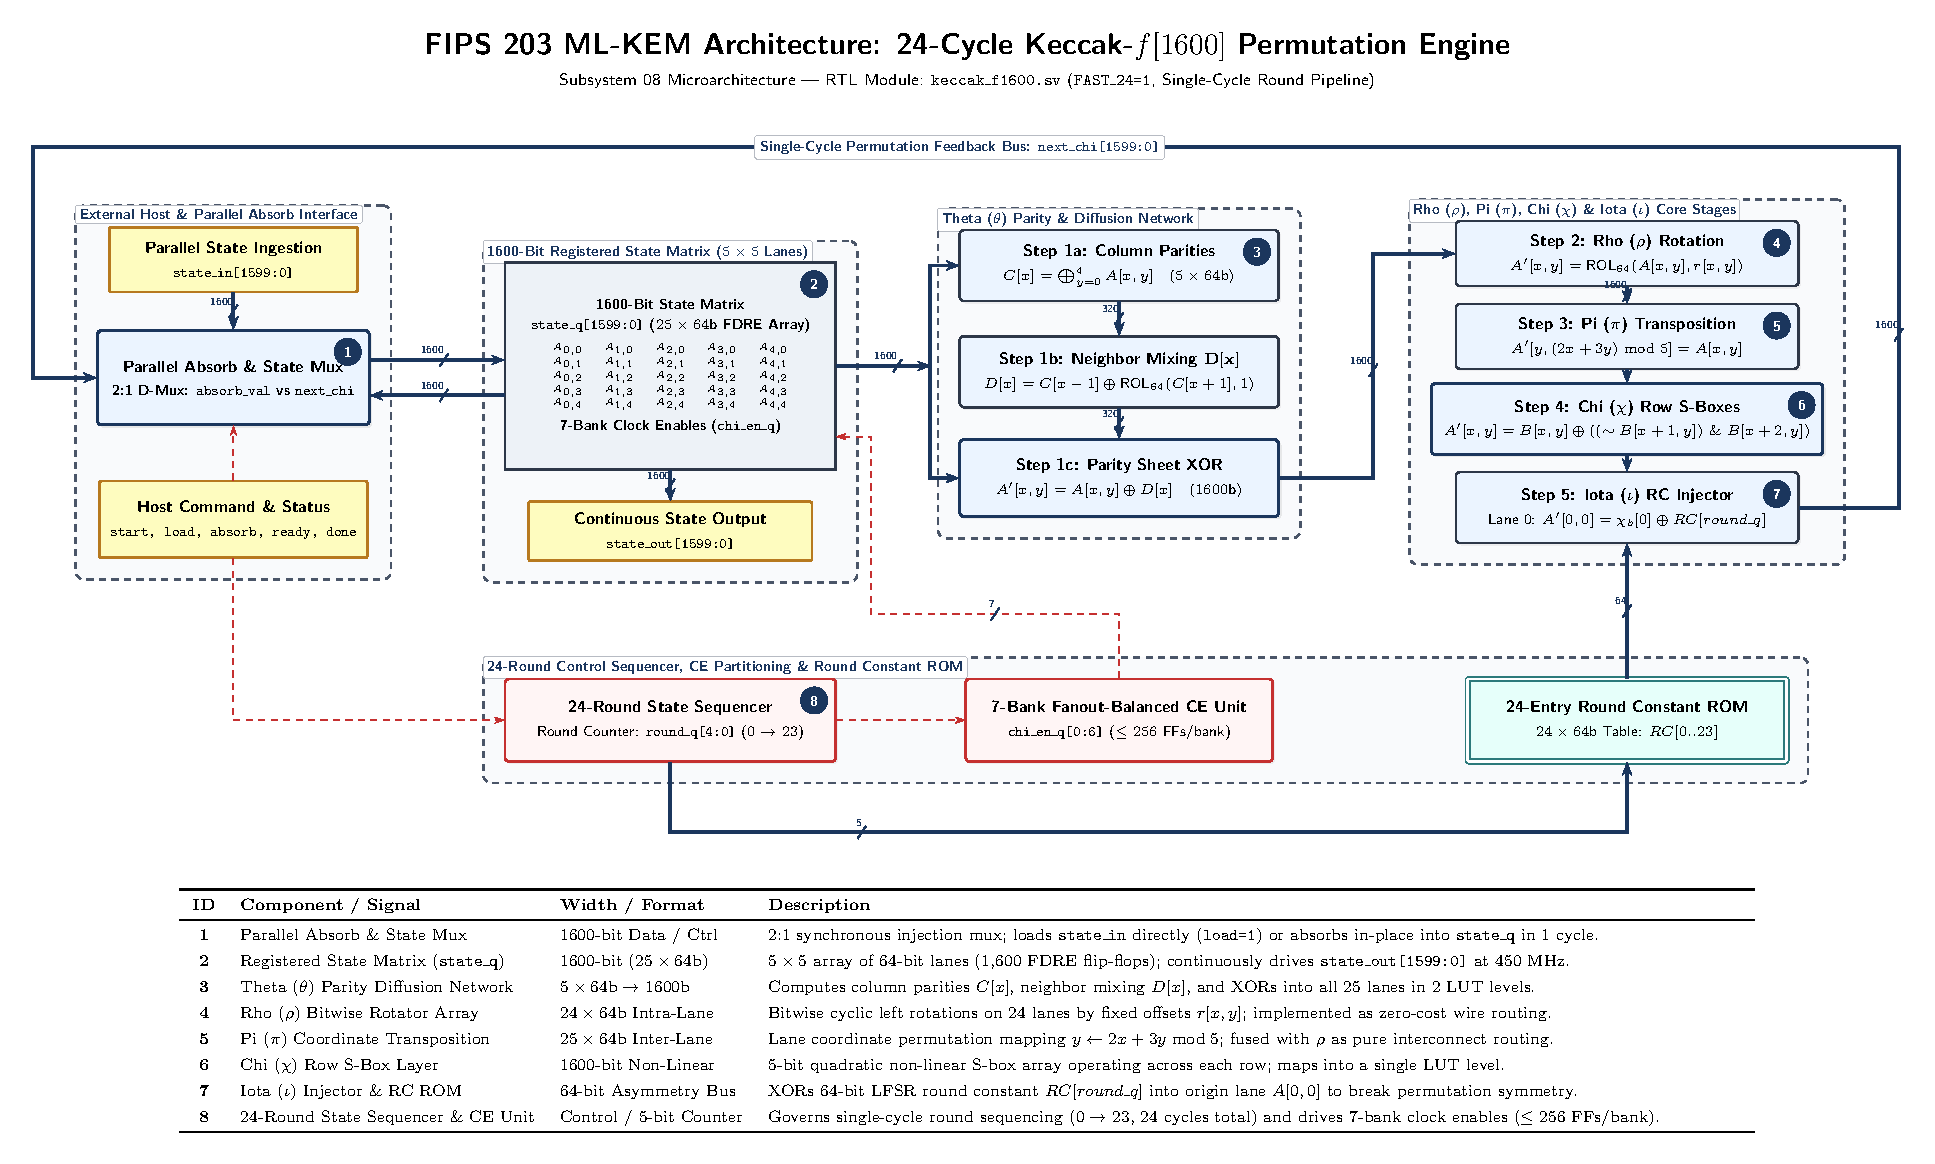
\includegraphics[width=\textwidth]{figures/fig08_keccak_f1600_core.pdf}
\caption{FIPS 203 \mbox{ML-KEM} Architecture: 24-Cycle Keccak-$f[1600]$ Permutation Engine (\texttt{keccak\_f1600.sv}). The datapath comprises an external host parallel ingestion and 2:1 multiplexer interface (\textbf{Callout~1}), a 1600-bit registered state matrix arranged as a $5 \times 5$ array of 64-bit lanes with 7-bank clock enables (\textbf{Callout~2}), a two-LUT-level column parity diffusion network $\theta$ (\textbf{Callout~3}), an intra-lane cyclic rotator array $\rho$ (\textbf{Callout~4}), an inter-lane coordinate transposition routing layer $\pi$ (\textbf{Callout~5}), a parallel 5-bit quadratic non-linear S-box layer $\chi$ (\textbf{Callout~6}), an LFSR-driven round constant asymmetry injector $\iota$ with 24-entry ROM (\textbf{Callout~7}), and a 24-round single-cycle state sequencer and fanout-balanced clock enable unit (\textbf{Callout~8}).}
\label{fig:keccak_core}
\end{figure*}

The microarchitecture of the 24-cycle Keccak-$f[1600]$ permutation core is illustrated in Fig.~\ref{fig:keccak_core}.

\subsubsection{1600-Bit State Geometry and Tensor Organization}
The internal state $S$ of Keccak-$f[1600]$ is mathematically formalized as a three-dimensional tensor over the Galois field $\mathbb{F}_2$:
\begin{equation}
\mathbf{A} \in \mathbb{F}_2^{5 \times 5 \times 64},
\label{eq:keccak_state_tensor}
\end{equation}
indexed by horizontal coordinate $x \in \mathbb{Z}_5 = \{0, 1, 2, 3, 4\}$, vertical coordinate $y \in \mathbb{Z}_5$, and bit position within each word $z \in \mathbb{Z}_{64} = \{0, 1, \dots, 63\}$. The aggregate state dimension is $b = 5 \times 5 \times 64 = 1600\text{ bits}$. Within the physical datapath, the state is structured into standard cryptographic sub-volumes:
\begin{itemize}
    \item \textbf{Lane $\mathbf{A}[x, y]$:} A 1D 64-bit vector at coordinate $(x, y)$, defined as $\mathbf{A}[x, y] = \sum_{z=0}^{63} \mathbf{A}[x, y, z] \cdot 2^z \in \mathbb{F}_2^{64}$;
    \item \textbf{Sheet $\mathbf{A}[x, *, *]$:} A 2D slice of dimension $5 \times 64 = 320\text{ bits}$ with fixed $x$;
    \item \textbf{Plane $\mathbf{A}[*, y, *]$:} A 2D slice of dimension $5 \times 64 = 320\text{ bits}$ with fixed $y$;
    \item \textbf{Column $\mathbf{A}[x, *, z]$:} A 1D 5-bit vector with fixed $(x, z)$;
    \item \textbf{Row $\mathbf{A}[*, y, z]$:} A 1D 5-bit vector with fixed $(y, z)$.
\end{itemize}

In the RTL module \texttt{keccak\_f1600.sv}, the state is mapped into a flattened 1600-bit register array \texttt{state\_q[1599:0]} using standard FIPS~202 little-endian lane serialization (\textbf{Callout~2}):
\begin{equation}
\text{bit\_index}(x, y, z) = 64 \cdot (5y + x) + z, \quad \text{lane\_index}(i) = 5y + x,
\label{eq:state_indexing}
\end{equation}
where lane $0$ occupies bits $[63:0]$ and lane $24$ occupies bits $[1599:1536]$.

\subsubsection{Microarchitecture of Round Transformations}
The Keccak-$f[1600]$ permutation applies 24 iterations ($i_r \in \{0, 1, \dots, 23\}$) of the composite round transformation $\text{Rnd}(\mathbf{A}, i_r)$:
\begin{equation}
\mathbf{A}^{(i_r+1)} = \text{Rnd}(\mathbf{A}^{(i_r)}, i_r) = (\iota \circ \chi \circ \pi \circ \rho \circ \theta)(\mathbf{A}^{(i_r)}).
\label{eq:keccak_round_composition}
\end{equation}
The five sequential step mappings are realized through specialized combinational logic structures:

\paragraph{Step 1: $\theta$ (Theta) --- Column Parity Diffusion}
Theta is a linear mapping over $\mathbb{F}_2$ (algebraic degree 1) that introduces rapid inter-column diffusion. For each column $x \in \mathbb{Z}_5$, the 64-bit column parity $C[x]$ is computed by XORing the five lanes across all rows (\textbf{Callout~3}):
\begin{equation}
C[x] = \bigoplus_{y=0}^4 \mathbf{A}[x, y] = \bigoplus_{y \in \mathbb{Z}_5} \mathbf{A}[x, y].
\label{eq:theta_c}
\end{equation}
Next, the neighbor mixing word $D[x]$ is formed by XORing the parity of the preceding column $(x-1) \bmod 5$ with the 1-bit circularly rotated parity of the succeeding column $(x+1) \bmod 5$:
\begin{equation}
D[x] = C[(x+4) \bmod 5] \oplus \text{ROL}_{64}(C[(x+1) \bmod 5], 1),
\label{eq:theta_d}
\end{equation}
where $\text{ROL}_{64}(X, n) = (X \ll n) \mid (X \gg (64 - n))$. Finally, $D[x]$ is XORed into every bit of the state:
\begin{equation}
\mathbf{A}'[x, y] = \mathbf{A}[x, y] \oplus D[x], \quad \forall x, y \in \mathbb{Z}_5.
\label{eq:theta_out}
\end{equation}
In hardware, each bit of $C[x]$ is a 5-input XOR that maps directly into a single 5-input Look-Up Table (\texttt{LUT5}). The subsequent computation of $D[x]$ and the XOR injection into $\mathbf{A}[x, y]$ is a 3-input XOR ($A \oplus C_{-1} \oplus \text{ROL}(C_{+1})$), mapping into a single \texttt{LUT3}. Consequently, the entire 1600-bit $\theta$ transformation evaluates in exactly \textbf{two LUT levels} ($\approx 80\text{ ps}$ logic delay).

\paragraph{Step 2: $\rho$ (Rho) --- Intra-Lane Cyclic Shifts}
Rho rotates the bits within each 64-bit lane by a fixed rotation constant $r[x, y] \in \{0, 1, \dots, 63\}$ (\textbf{Callout~4}):
\begin{equation}
\mathbf{A}'[x, y] = \text{ROL}_{64}(\mathbf{A}[x, y], r[x, y]).
\label{eq:rho_step}
\end{equation}
For lane $(0, 0)$, $r[0, 0] = 0$. The remaining 24 offsets are defined by the recurrence $\begin{pmatrix} x \\ y \end{pmatrix}_{t+1} = \begin{pmatrix} 0 & 1 \\ 2 & 3 \end{pmatrix} \begin{pmatrix} x \\ y \end{pmatrix}_t \pmod 5$ with $r[x, y] = \frac{(t+1)(t+2)}{2} \bmod 64$ for $t \in \{0, \dots, 23\}$.

\paragraph{Step 3: $\pi$ (Pi) --- Inter-Lane Coordinate Transposition}
Pi permutes the spatial positions of lanes within the $5 \times 5$ plane without altering bit order (\textbf{Callout~5}):
\begin{equation}
\mathbf{A}'[y, (2x + 3y) \bmod 5] = \mathbf{A}[x, y].
\label{eq:pi_step}
\end{equation}

\paragraph{Fused Wire Permutation ($\pi \circ \rho$)}
In \texttt{keccak\_f1600.sv}, steps $\rho$ and $\pi$ are fused into a single recurrence loop (\texttt{GEN\_B}):
\begin{equation}
B[y, (2x + 3y) \bmod 5] = \text{ROL}_{64}(\mathbf{A}[x, y], r[x, y]).
\label{eq:fused_pi_rho}
\end{equation}
Because the rotation offsets $r[x, y]$ and coordinate mappings $\pi(x, y)$ are static constants known at elaboration time, the combined $\pi \circ \rho$ transformation requires \textbf{zero LUTs, zero logic gates, and zero propagation delay}, synthesizing entirely as hardwired metal wire routing between the $\theta$ outputs and the $\chi$ inputs.

\paragraph{Step 4: $\chi$ (Chi) --- Non-Linear Row Inversion}
Chi is the sole non-linear transformation in Keccak-$f[1600]$. Operating row-wise across each column $x \in \mathbb{Z}_5$ for all $y \in \mathbb{Z}_5$ (\textbf{Callout~6}):
\begin{equation}
\begin{aligned}
\mathbf{A}'[x, y] &= B[x, y] \oplus ((\sim B[(x+1) \bmod 5, y]) \\
                  &\quad \ \& \ B[(x+2) \bmod 5, y]).
\end{aligned}
\label{eq:chi_step}
\end{equation}
Chi acts as an array of 320 parallel 5-bit non-linear S-boxes ($\chi: \mathbb{F}_2^5 \to \mathbb{F}_2^5$) with algebraic degree 2. Each bit requires one 2-input AND, one inverter, and one 2-input XOR. In the AMD UltraScale CLB architecture, this 3-input Boolean function maps into a single Look-Up Table (\texttt{LUT3} or \texttt{LUT6}).

\paragraph{Step 5: $\iota$ (Iota) --- Round Constant Asymmetry Addition}
Iota breaks the rotational and translational symmetry of the permutation by XORing a 64-bit round constant $RC[i_r]$ into origin lane $(0, 0)$ (\textbf{Callout~7}):
\begin{align}
\mathbf{A}'[0, 0] &= \mathbf{A}[0, 0] \oplus RC[i_r], \label{eq:iota_step} \\
\mathbf{A}'[x, y] &= \mathbf{A}[x, y], \quad \forall (x, y) \neq (0, 0). \nonumber
\end{align}
The round constants $RC[i_r]$ contain non-zero bits only at positions $2^j - 1$ ($j \in \{0, \dots, 6\}$), generated by a degree-8 Linear Feedback Shift Register (\mbox{LFSR}) with characteristic polynomial $P(x) = x^8 + x^6 + x^5 + x^4 + 1$. In RTL, $RC[i_r]$ is driven by a 64-bit lookup function \texttt{rc(round\_q[4:0])}. For lane 0, synthesis folds the $\chi$ expression, the round constant XOR, and the state multiplexer into a \textbf{single 6-input LUT (\texttt{LUT6})}.

\begin{algorithm}[!t]
\caption{Single-Round Keccak-$f[1600]$ Transformation $\text{Rnd}(\mathbf{A}, i_r)$}
\label{alg:keccak_round}
\begin{algorithmic}[1]
\Require State array $\mathbf{A} \in \mathbb{F}_2^{5 \times 5 \times 64}$, Round index $i_r \in \{0, \dots, 23\}$
\Ensure Updated state array $\mathbf{A}' \in \mathbb{F}_2^{5 \times 5 \times 64}$
\For{$x = 0$ to $4$} \Comment{Step 1a: Column Parities}
    \State $C[x] \leftarrow \mathbf{A}[x, 0] \oplus \mathbf{A}[x, 1] \oplus \mathbf{A}[x, 2] \oplus \mathbf{A}[x, 3] \oplus \mathbf{A}[x, 4]$
\EndFor
\For{$x = 0$ to $4$} \Comment{Step 1b: Neighbor Mixing}
    \State $D[x] \leftarrow C[(x+4) \bmod 5] \oplus \text{ROL}_{64}(C[(x+1) \bmod 5], 1)$
\EndFor
\For{$x = 0$ to $4, \; y = 0$ to $4$} \Comment{Step 1c: Parity Sheet XOR}
    \State $\mathbf{A}_\theta[x, y] \leftarrow \mathbf{A}[x, y] \oplus D[x]$
\EndFor
\For{$x = 0$ to $4, \; y = 0$ to $4$} \Comment{Steps 2 \& 3: Fused Rho + Pi}
    \State $B[y, (2x + 3y) \bmod 5] \leftarrow \text{ROL}_{64}(\mathbf{A}_\theta[x, y], r[x, y])$
\EndFor
\For{$x = 0$ to $4, \; y = 0$ to $4$} \Comment{Step 4: Non-Linear Chi S-Box}
    \State $\mathbf{A}_\chi[x, y] \leftarrow B[x, y] \oplus ((\sim B[(x+1) \bmod 5, y]) \ \& \ B[(x+2) \bmod 5, y])$
\EndFor
\State $\mathbf{A}'[0, 0] \leftarrow \mathbf{A}_\chi[0, 0] \oplus RC[i_r]$ \Comment{Step 5: Iota Constant Injection}
\For{$(x, y) \neq (0, 0)$}
    \State $\mathbf{A}'[x, y] \leftarrow \mathbf{A}_\chi[x, y]$
\EndFor
\State \Return $\mathbf{A}'$
\end{algorithmic}
\end{algorithm}

\subsubsection{Single-Round Architecture (\texttt{FAST\_24 = 1}) and Dual-Phase Mode}
The core supports a top-level architectural parameter:
\begin{equation}
\texttt{parameter bit FAST\_24 = 1}
\end{equation}
When \texttt{FAST\_24 = 1} (the production configuration in our accelerator), all five step transformations ($\theta \to \rho \to \pi \to \chi \to \iota$) evaluate combinatorially within a \textbf{single clock cycle}. The intermediate register \texttt{theta\_q[1599:0]} is bypassed via \texttt{assign theta\_wire = next\_theta;}, allowing logic synthesis to optimize away all 1600 intermediate flip-flops. The permutation terminates in exactly \textbf{24 clock cycles} ($53.33\text{ ns}$ at $450.0\text{ MHz}$).

When \texttt{FAST\_24 = 0}, each round is decomposed into two phases: Phase 0 registers $\theta$ into \texttt{theta\_q}, and Phase 1 executes $\rho$-$\pi$-$\chi$-$\iota$ into \texttt{state\_q}, completing in 48 clock cycles. This cuts the combinational path in half, enabling operation beyond $600\text{ MHz}$ or easing timing closure on lower-speed FPGA fabrics.

\subsubsection{Parallel 1600-Bit Absorb Multiplexer with In-Place XOR Injection}
Conventional sponge accelerators suffer from multi-cycle absorption overheads because message words must be loaded sequentially into state registers. As detailed in \textbf{Callout~1} of Fig.~\ref{fig:keccak_core}, \texttt{keccak\_f1600.sv} eliminates this latency by embedding a 1600-bit XOR injection multiplexer directly into the D-input stage of the state flip-flops:
\begin{align}
\texttt{abs\_val}[i] &= (\texttt{first} \ ? \ 0 : \texttt{state}[i]) \oplus \texttt{in}[i], \label{eq:absorb_val} \\
\texttt{state\_d}[i] &= \texttt{absorb\_en} \ ? \ \texttt{abs\_val}[i] : \texttt{next\_chi}[i]. \label{eq:state_d}
\end{align}
This provides three distinct zero-overhead operating modes:
\begin{itemize}
    \item \textbf{Direct Parallel Load (\texttt{load = 1}):} Injects $\texttt{state\_in}$ directly into $\texttt{state\_q}$ in a single cycle while forcing feedback to zero, providing instantaneous state initialization;
    \item \textbf{Sponge Accumulation (\texttt{absorb = 1, absorb\_first = 0}):} Computes $S_{\text{new}} \leftarrow S_{\text{current}} \oplus \texttt{state\_in}$ in a single clock cycle, absorbing rate-delimited message blocks (1088b or 1344b) instantaneously;
    \item \textbf{Autonomous Permutation Feedback (\texttt{absorb\_en = 0}):} Connects the round output $\texttt{next\_chi}$ directly back to $\texttt{state\_q}$, iterating round-by-round with zero multiplexer overhead.
\end{itemize}

\subsubsection{Timing Optimization for 450 MHz: Critical Path and 7-Bank Clock Enables}
To achieve timing closure at $T_{\text{clk}} = 2.222\text{ ns}$ ($450.0\text{ MHz}$) across a 1600-bit wide iterative register array, the datapath combinational logic depth was strictly capped at \textbf{3 LUT levels}:
\begin{equation}
\begin{aligned}
\text{Logic Depth} &= \underbrace{\text{GEN\_C}}_{1\text{ (LUT5)}} + \underbrace{\text{GEN\_THETA}}_{1\text{ (LUT3)}} \\
&\quad + \underbrace{\text{GEN\_B}}_{0\text{ (Routing)}} + \underbrace{\text{GEN\_CHI/MUX}}_{1\text{ (LUT6)}} = 3\text{ levels}.
\end{aligned}
\label{eq:lut_depth}
\end{equation}

Driving a single global enable net across 1,600 flip-flops incurs massive routing delays ($t_{\text{net}} > 2.0\text{ ns}$) spanning dozens of CLB columns. The proposed permutation core resolves this by partitioning the 25 lanes into \textbf{7 fanout-balanced clusters} driven by localized enable registers \texttt{chi\_en\_q[0:6]} (\textbf{Callout~8}):
\begin{equation}
\texttt{state\_ce}[i] = \texttt{absorb\_en} \mid \texttt{chi\_en\_q}[\lfloor i / 4 \rfloor],
\label{eq:ce_partition}
\end{equation}
evaluated for all $i \in [0, 24]$, capping the physical load of each clock-enable net to $\le 256$ flip-flops ($4 \times 64\text{ FFs}$ for banks $0 \dots 5$, and $64\text{ FFs}$ for bank 6). Furthermore, when the engine is idle ($\texttt{busy\_q} = 0$), all seven \texttt{chi\_en\_q} registers deassert, completely freezing switching activity across all 1600 state flip-flops and eliminating dynamic power dissipation between sponge operations.

% ==============================================================================
% Subsection VI-C: High-Bandwidth 64-Bit Lane Absorb Interface & Squeeze Buffer
% ==============================================================================
\subsection{High-Bandwidth 64-Bit Lane Absorb Interface and Elastic Squeeze Buffer}
\label{sec:lane_absorb}

\begin{figure*}[!t]
\centering
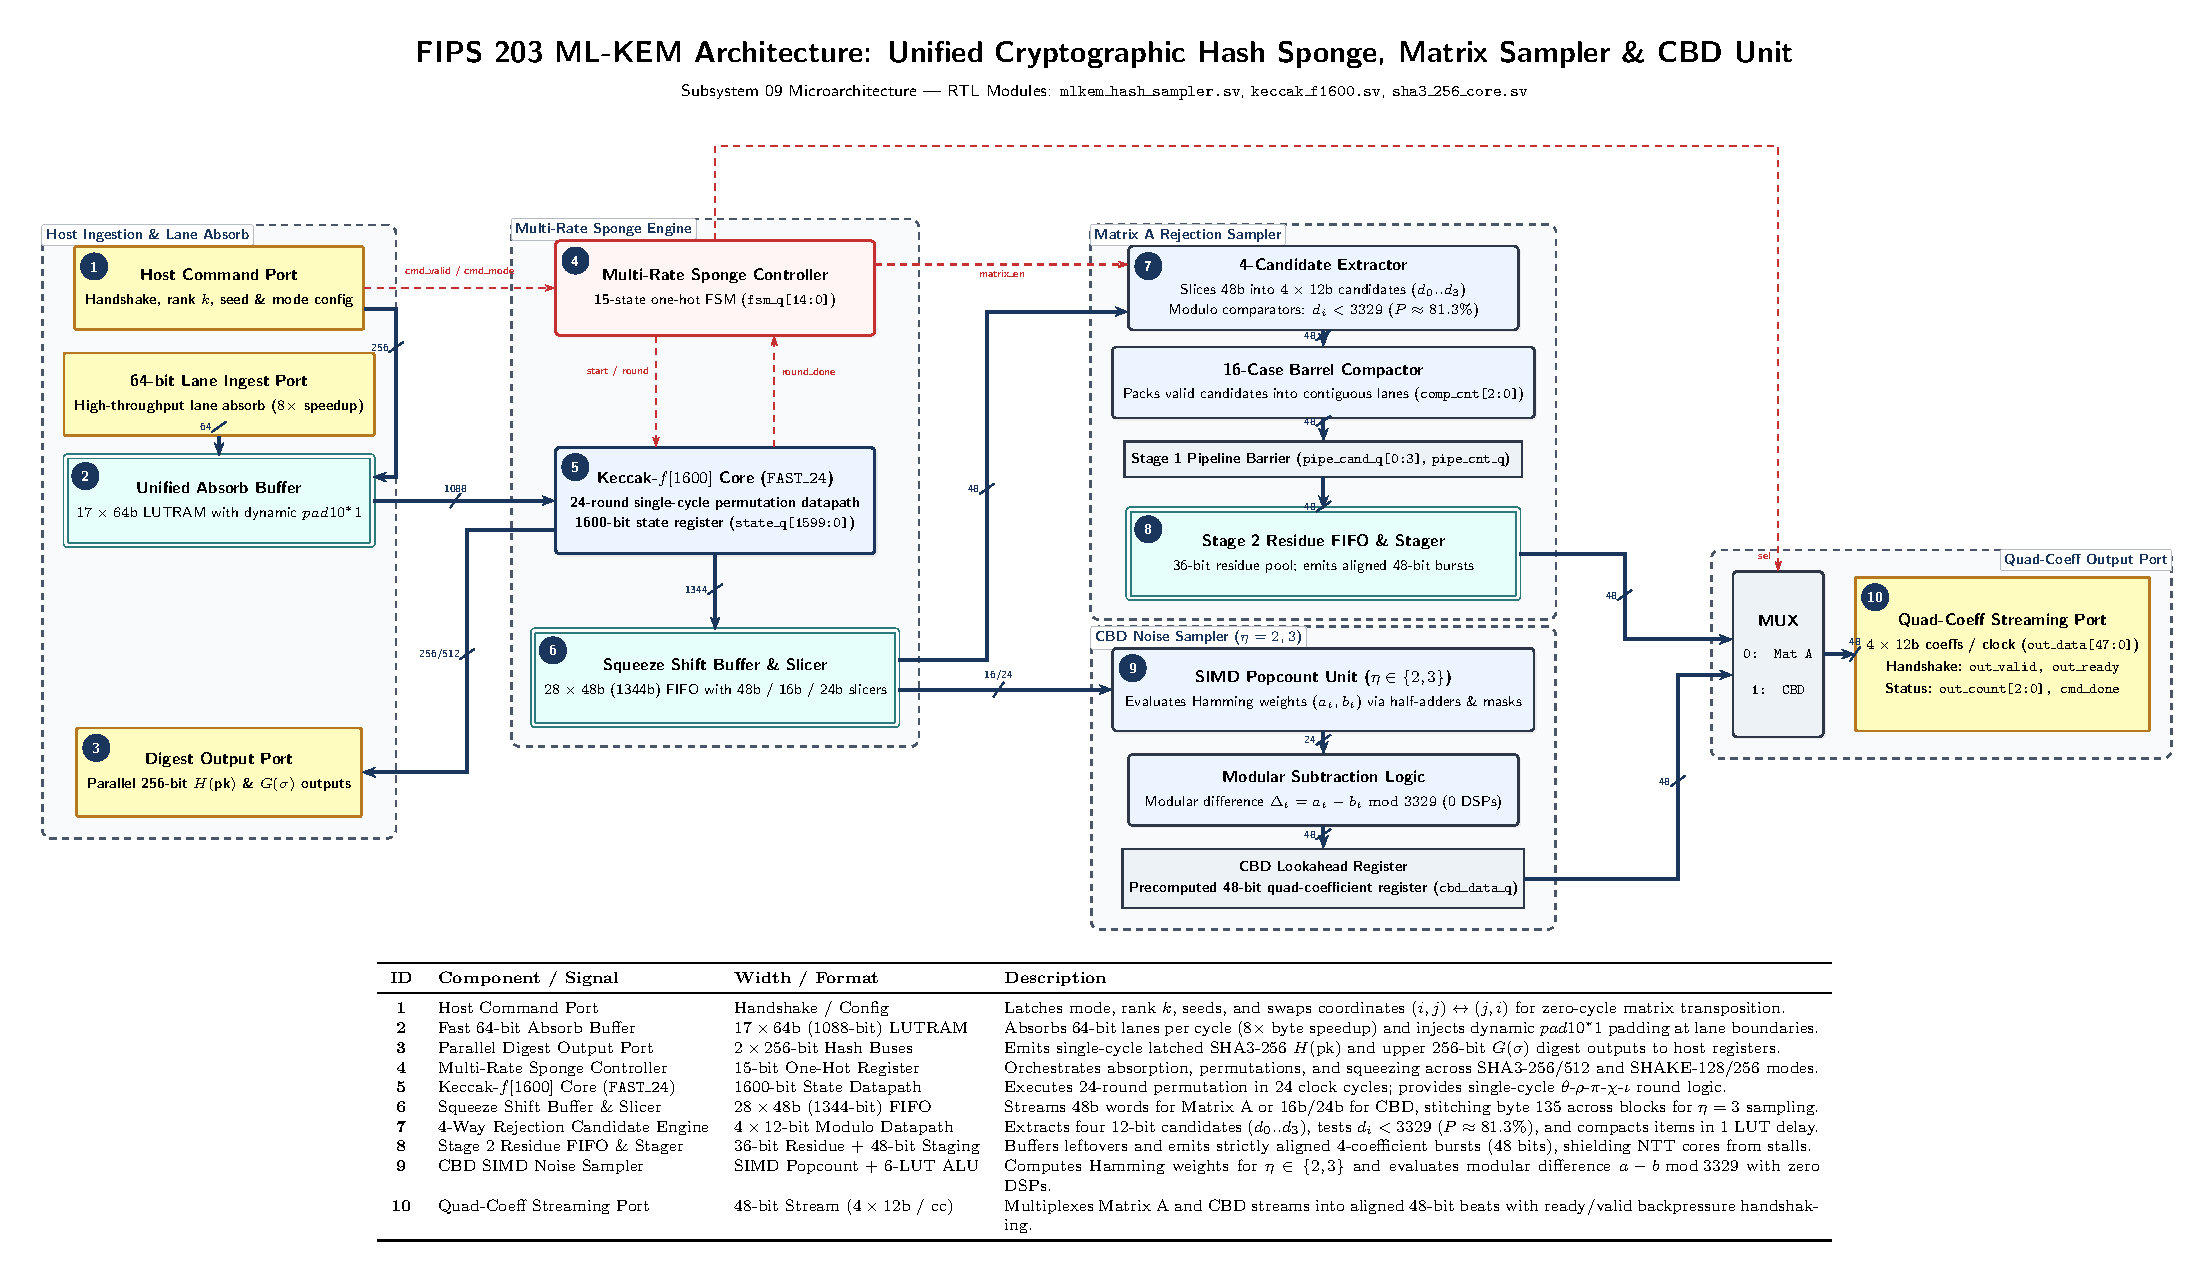
\includegraphics[width=\textwidth]{figures/fig09_hash_sampler_cbd.pdf}
\caption{FIPS 203 \mbox{ML-KEM} Architecture: Unified Cryptographic Hash Sponge, Matrix Sampler and CBD Unit (\texttt{mlkem\_hash\_sampler.sv}). The architecture integrates a host command port with zero-cycle matrix transposition (\textbf{Callout~1}), a fast 64-bit absorb buffer with dynamic $pad10^*1$ padding (\textbf{Callout~2}), parallel 256-bit digest output ports (\textbf{Callout~3}), a 15-state one-hot multi-rate sponge controller (\textbf{Callout~4}), a single-round 24-cycle Keccak-$f[1600]$ engine (\textbf{Callout~5}), a 1344-bit multi-rate squeeze shift buffer and slicer (\textbf{Callout~6}), a 4-way rejection candidate modulo engine (\textbf{Callout~7}), a Stage 2 residue FIFO and 48-bit stager (\textbf{Callout~8}), a SIMD bit-mask CBD noise sampler with 6-LUT modular subtractors (\textbf{Callout~9}), and a decoupled quad-coefficient streaming port (\textbf{Callout~10}).}
\label{fig:hash_sampler_cbd}
\end{figure*}

The microarchitecture of the unified cryptographic hash sampler, rejection sampler, and CBD noise engine is detailed in Fig.~\ref{fig:hash_sampler_cbd}.

\subsubsection{Unified Multi-Mode Sponge Architecture and 15-State One-Hot Controller}
Rather than instantiating redundant Keccak cores for different functions, \texttt{mlkem\_hash\_sampler.sv} consolidates all cryptographic hashing and polynomial sampling requirements into a single shared Keccak-$f[1600]$ engine (\textbf{Callout~5}). The operational mode is selected via \texttt{cmd\_mode[2:0]} across six dedicated modes:
\begin{itemize}
    \item \textbf{Mode 0 (\texttt{SHA256}):} SHA3-256 ($r=1088, c=512$, domain \texttt{0x06}) for public key transcript hashing $H(ek)$ and message digest derivation $H(m)$;
    \item \textbf{Mode 1 (\texttt{SHA512}):} SHA3-512 ($r=576, c=1024$, domain \texttt{0x06}) for key derivation $G(\cdot)$ and shared secret expansion;
    \item \textbf{Mode 2 (\texttt{MATRIX}):} SHAKE-128 ($r=1344, c=256$, domain \texttt{0x1F}) for public matrix $\hat{\mathbf{A}} \in \mathcal{T}_q^{k \times k}$ generation via on-the-fly rejection sampling (\texttt{SampleNTT} / \texttt{Parse});
    \item \textbf{Mode 3 (\texttt{VECTOR}):} SHAKE-256 ($r=1088, c=512$, domain \texttt{0x1F}) for secret and error noise vector sampling ($\mathbf{s}, \mathbf{e}, \mathbf{r}, \mathbf{e}_1, e_2$) via Centered Binomial Distribution (\texttt{SamplePolyCBD}$_\eta$);
    \item \textbf{Mode 4 (\texttt{SHAKE256}):} SHAKE-256 ($r=1088, c=512$, domain \texttt{0x1F}) for implicit rejection key derivation $J(z \parallel c, 32)$;
    \item \textbf{Mode 5 (\texttt{SHA512\_64}):} Fast 64-byte SHA3-512 mode for joint derivation $G(m \parallel H(ek))$, loading two 256-bit seed registers in parallel in a single clock cycle.
\end{itemize}

To guarantee timing closure at $450.0\text{ MHz}$, the control path is implemented as an explicit \textbf{15-state one-hot finite state machine} (\texttt{fsm\_q[14:0]}, \textbf{Callout~4}) with a permanent VCC clock-enable. Every state transition resolves within a single LUT delay, eliminating multi-level state decoding logic from critical handshake paths.

\subsubsection{High-Throughput 64-Bit Lane Absorb Interface (\texorpdfstring{$8\times$}{8x} Speedup)}
A severe performance bottleneck in conventional Keccak hardware implementations is byte-serial absorption. In \mbox{ML-KEM}, absorbing a public key $ek$ ($800\text{ B}$ for $k=2$, $1184\text{ B}$ for $k=3$, and $1568\text{ B}$ for $k=4$) byte-serially consumes up to 1,568 clock cycles solely for data ingestion.

The proposed sampler eliminates this bottleneck through the \textbf{Fast 64-Bit Lane Absorption Datapath} (\textbf{Callout~2}):
\begin{itemize}
    \item \textbf{Merged Single Absorb Buffer:} A unified $17 \times 64\text{-bit}$ register array \texttt{absorb\_buf\_q[0:16]} (1088 bits) services both byte-serial and 64-bit lane modes. In lane mode, 64-bit words are clocked directly into individual lane registers in a single cycle using one-hot write enables:
    \begin{equation}
    \begin{aligned}
    \texttt{lane\_we}[b] &= \texttt{fsm}[S\_LANE] \\
    &\quad \ \& \ \texttt{in\_valid} \ \& \ \texttt{sel}[b];
    \end{aligned}
    \label{eq:lane_we}
    \end{equation}
    \item \textbf{On-the-Fly Dynamic Padding:} Combinatorial multiplexer logic \texttt{lane\_block\_val} constructs the 1088-bit block dynamically. On the terminal message block (\texttt{in\_last\_block = 1}), it injects domain padding (\texttt{0x06} or \texttt{0x1F}) at the lane boundary defined by \texttt{in\_rem\_lanes[4:0]} and appends the terminal bit \texttt{0x8000\_0000\_0000\_0000} at lane 16;
    \item \textbf{Throughput Acceleration:} A full 136-byte block (17 lanes) absorbs in \textbf{17 clock cycles instead of 136 cycles}---an exact \textbf{$8\times$ absorption speedup};
    \item \textbf{Parallel Digest Buses:} Upon permutation completion, the 256-bit hash digest is latched immediately onto \texttt{digest\_out[255:0]} (\textbf{Callout~3}). In SHA3-512 mode, the upper 256 bits are simultaneously presented on \texttt{digest\_out\_sigma[255:0]}, enabling single-cycle key extraction without serial read-out cycles.
\end{itemize}

\subsubsection{Accelerated Joint Derivation \texorpdfstring{$G(m \parallel H(ek))$}{G(m || H(ek))} (Mode 5)}
During encapsulation and decapsulation re-encryption, the accelerator computes $(K, r) \leftarrow \text{SHA3-512}(m \parallel H(ek))$. The input message is exactly 64 bytes ($32\text{ B}$ message $m$ concatenated with $32\text{ B}$ public key hash $H(ek)$), fitting entirely within a single SHA3-512 rate block ($r = 72\text{ bytes}$).

Mode 5 (\texttt{SHA512\_64}) optimizes this operation:
\begin{enumerate}
    \item Input registers \texttt{cmd\_seed} ($m$) and \texttt{cmd\_seed\_hi} ($H(ek)$) are loaded directly into the Keccak state buffer in parallel in \textbf{exactly 1 clock cycle} in state \texttt{S\_START}, along with domain padding (\texttt{0x06}) and terminal bit (\texttt{0x80});
    \item Permutation executes in 24 clock cycles in state \texttt{S\_WAIT0};
    \item On cycle 25, the 256-bit shared key $K$ is presented on \texttt{digest\_out[255:0]} while the 256-bit coin seed $r$ is simultaneously presented on \texttt{digest\_out\_sigma[255:0]};
    \item Total derivation latency: exactly \textbf{25 clock cycles}, eliminating 64 cycles of serial message absorption and 64 cycles of serial digest reading.
\end{enumerate}

% ==============================================================================
% Subsection VI-D: Uniform Rejection Sampler for Public Matrix A
% ==============================================================================
\subsection{Uniform Rejection Sampler for Public Matrix \texorpdfstring{$\hat{\mathbf{A}}$}{A}}
\label{sec:matrix_sampler}

In FIPS~203, each entry $\hat{\mathbf{A}}[i, j]$ of the public matrix is derived by absorbing a 34-byte seed $M_{i, j} = \rho \parallel j \parallel i$ into SHAKE-128 and squeezing pseudorandom bytes. The `Parse` algorithm partitions every 3 contiguous squeezed bytes $(B_0, B_1, B_2)$ into two 12-bit integer candidates $d_1, d_2 \in [0, 4095]$:
\begin{align}
d_1 &= B_0 + 256 \cdot (B_1 \bmod 16) = B_0 \mid ((B_1 \ \& \ \texttt{0x0F}) \ll 8), \label{eq:parse_d1} \\
d_2 &= \lfloor B_1 / 16 \rfloor + 16 \cdot B_2 = (B_1 \gg 4) \mid (B_2 \ll 4). \label{eq:parse_d2}
\end{align}

\subsubsection{Acceptance Probability and Negative Binomial Analysis}
A candidate $d$ is accepted if and only if $d < q = 3329$. Because squeezed bits are uniformly distributed over $\{0, 1\}^{12}$, the acceptance probability $P_{\text{acc}}$ is:
\begin{align}
P_{\text{acc}} &= \frac{3329}{4096} \approx 0.812744 \quad (81.27\%), \label{eq:rejection_prob} \\
P_{\text{rej}} &= 1 - P_{\text{acc}} = \frac{767}{4096} \approx 0.187256 \quad (18.73\%). \nonumber
\end{align}
To accumulate $n = 256$ valid ring coefficients, the expected number of 12-bit candidates $\mathbb{E}[M]$ and squeezed bytes $\mathbb{E}[N_{\text{bytes}}]$ are:
\begin{align}
\mathbb{E}[M] &= \frac{256}{P_{\text{acc}}} \approx 314.98\text{ candidates}, \label{eq:expected_candidates} \\
\mathbb{E}[N_{\text{bytes}}] &= \frac{3}{2} \cdot \mathbb{E}[M] \approx 472.47\text{ bytes}. \nonumber
\end{align}
Each SHAKE-128 squeeze block delivers $r = 168\text{ bytes}$ ($1344\text{ bits}$), yielding exactly $168 \times (2/3) = 112$ candidates. Across sequential squeeze blocks:
\begin{itemize}
    \item Block 1 (112 candidates): $\mathbb{E}[\text{accepted}] = 91.03$ coefficients;
    \item Block 2 (224 candidates): $\mathbb{E}[\text{accepted}] = 182.05$ coefficients;
    \item Block 3 (336 candidates): $\mathbb{E}[\text{accepted}] = 273.08$ coefficients ($> 256$).
\end{itemize}
The cumulative probability that three squeeze blocks fail to yield 256 coefficients is:
\begin{equation}
\begin{aligned}
P(X < 256 \mid N=336) &= \sum_{k=0}^{255} \binom{336}{k} p^k (1-p)^{336-k} \\
&\approx 8.33 \times 10^{-3} \quad (0.833\%).
\end{aligned}
\label{eq:cumulative_binomial}
\end{equation}
Thus, exactly 3 squeeze blocks suffice in $99.167\%$ of cases. For the remaining $0.833\%$, the FSM seamlessly transitions from \texttt{S\_MATRIX\_SCAN} into \texttt{S\_MATRIX\_MORE} to squeeze a 4th block without corrupting the pipeline.

\subsubsection{Two-Stage Decoupled Rejection Pipeline}
To sustain maximum throughput and match the 4-way Stockham NTT datapath, the rejection sampler processes \textbf{four 12-bit candidates (48 bits) per clock cycle} through a two-stage decoupled pipeline (\textbf{Callouts~7 and~8}):
\begin{itemize}
    \item \textbf{Step 1: 4-Candidate Extraction and Parallel Modulo Comparison:} A 48-bit word (6 bytes) from \texttt{stream\_buf} is sliced into four 12-bit candidates $d_0 \dots d_3$ (\textbf{Callout~7}). Four parallel 12-bit unsigned comparators evaluate $\texttt{cand\_valid}[i] = (d_i < 3329)$;
    \item \textbf{Step 2: Constant-Depth 16-Case Barrel Compaction:} A single-LUT-level multiplexer evaluates the 16 possible acceptance bitmasks $\{\texttt{cand\_valid}[3:0]\}$ and packs valid candidates contiguously into \texttt{comp\_cand[0:3]}, generating valid count $\texttt{comp\_cnt} \in \{0, \dots, 4\}$;
    \item \textbf{Step 3: Stage 1 Pipeline Registration:} Registers \texttt{pipe\_cand\_q[0:3]} and \texttt{pipe\_cnt\_q} latch the compacted candidates, breaking the long combinational path between the Keccak state buffer and the output accumulator;
    \item \textbf{Step 4: Stage 2 36-Bit Residue FIFO and 48-Bit Staging Register:} Because rejection is stochastic, the arrival count varies ($0 \dots 4$). A 36-bit residue accumulator \texttt{residue\_q[35:0]} stores up to 3 leftover coefficients ($\texttt{residue\_cnt\_q} \in \{0, 1, 2, 3\}$, \textbf{Callout~8}). When the total available candidates $\text{total\_avail} = \texttt{residue\_cnt\_q} + \texttt{pipe\_cnt\_q} \ge 4$, exactly four coefficients are packed into \texttt{stage\_data\_q[47:0]} and \texttt{stage\_valid\_q} asserts high, while leftover candidates ($\text{total\_avail} - 4$) are retained in \texttt{residue\_q}.
\end{itemize}
This guarantees that every beat on \texttt{mat\_out\_valid} delivers \textbf{strictly four aligned 12-bit coefficients (48 bits)}, completely shielding the downstream NTT cores from rejection stalls and bubble cycles.

\begin{algorithm}[!t]
\caption{Pipelined 4-Way Rejection Sampling and Residue Packing}
\label{alg:rejection_sampling}
\begin{algorithmic}[1]
\Require 48-bit word $W$ from \texttt{stream\_buf}, Residue \texttt{residue\_q[35:0]}, Count $\texttt{residue\_cnt\_q} \in \{0, 1, 2, 3\}$
\Ensure Aligned quad data \texttt{stage\_data\_q[47:0]}, \texttt{stage\_valid\_q}, Updated residue
\State $d_0 \leftarrow W[11:0], \; d_1 \leftarrow W[23:12], \; d_2 \leftarrow W[35:24], \; d_3 \leftarrow W[47:36]$
\For{$i = 0$ to $3$} \Comment{Parallel Modulo Comparison}
    \State $\texttt{cand\_valid}[i] \leftarrow (d_i < 3329)$
\EndFor
\State $(\texttt{comp\_cand}[0:3], \texttt{comp\_cnt}) \leftarrow \text{Compact}_{16}(d_{0..3}, \texttt{cand\_valid}_{0..3})$
\State $\text{total\_avail} \leftarrow \texttt{residue\_cnt\_q} + \texttt{comp\_cnt}$ \Comment{Pool candidates ($0 \dots 7$)}
\State $\text{pool} \leftarrow \text{Concat}(\texttt{residue\_q}[12 \cdot \texttt{residue\_cnt\_q} - 1 : 0], \; \texttt{comp\_cand}[0 : \texttt{comp\_cnt} - 1])$
\If{$\text{total\_avail} \ge 4$}
    \State $\texttt{stage\_data\_q} \leftarrow \{\text{pool}[3], \text{pool}[2], \text{pool}[1], \text{pool}[0]\}$
    \State $\texttt{stage\_valid\_q} \leftarrow 1$
    \State $\texttt{residue\_q} \leftarrow \text{pool}[\text{total\_avail} - 1 : 4]$
    \State $\texttt{residue\_cnt\_q} \leftarrow \text{total\_avail} - 4$
\Else
    \State $\texttt{stage\_valid\_q} \leftarrow 0$
    \State $\texttt{residue\_q} \leftarrow \text{pool}[\text{total\_avail} - 1 : 0]$
    \State $\texttt{residue\_cnt\_q} \leftarrow \text{total\_avail}$
\EndIf
\end{algorithmic}
\end{algorithm}

\subsubsection{Zero-Overhead On-the-Fly Matrix Transposition (\texttt{cmd\_transpose})}
During \mbox{ML-KEM} Encapsulation, matrix-vector multiplication requires the transpose of the public matrix: $\hat{\mathbf{u}} = \hat{\mathbf{A}}^T \hat{\mathbf{r}} + \mathbf{e}_1$. Instead of storing the $k \times k$ polynomial matrix in Block RAM and executing an expensive matrix transpose routine, the proposed sampler transposes on the fly (\textbf{Callout~1}). The control input \texttt{cmd\_transpose} swaps the coordinate bytes injected into the SHAKE-128 initial state:
\begin{align}
\texttt{init\_byte32} &= \begin{cases} \{5\text{'b}0, \texttt{row\_q}\}, & \text{if } \texttt{cmd\_trans} \\ \{5\text{'b}0, \texttt{col\_q}\}, & \text{otherwise} \end{cases} \label{eq:transpose_byte32} \\
\texttt{init\_byte33} &= \begin{cases} \{5\text{'b}0, \texttt{col\_q}\}, & \text{if } \texttt{cmd\_trans} \\ \{5\text{'b}0, \texttt{row\_q}\}, & \text{otherwise} \end{cases} \label{eq:transpose_byte33}
\end{align}
Transposition incurs \textbf{zero clock cycles and zero additional memory overhead}.

% ==============================================================================
% Subsection VI-E: Centered Binomial Distribution (CBD) Sampler
% ==============================================================================
\subsection{Centered Binomial Distribution (\texorpdfstring{$\text{CBD}_\eta$}{CBD\_eta}) Noise Sampler}
\label{sec:cbd_sampler}

The secret and error noise vectors are sampled from the Centered Binomial Distribution $\mathcal{D}_\eta(\mathcal{R}_q)$ for $\eta \in \{2, 3\}$. Squeezing $64\eta$ bytes from SHAKE-256, each coefficient $f_i$ is computed from $2\eta$ uniform bits $(a_0 \dots a_{\eta-1}, b_0 \dots b_{\eta-1})$:
\begin{equation}
f_i = \sum_{j=0}^{\eta-1} a_j - \sum_{j=0}^{\eta-1} b_j \pmod q.
\label{eq:cbd_math}
\end{equation}

\subsubsection{SIMD Bit-Mask Popcount Datapath}
The CBD engine generates four coefficients per clock cycle deterministically (\textbf{Callout~9}):
\begin{itemize}
    \item \textbf{For $\eta = 2$ (\mbox{ML-KEM-768/1024}):} Each coefficient consumes $2\eta = 4\text{ bits}$. A 16-bit word $w \in \{0, 1\}^{16}$ yields four coefficients: $a = w[4t] + w[4t+1]$ and $b = w[4t+2] + w[4t+3]$ ($t \in \{0, \dots, 3\}$), evaluated using parallel 2-bit half-adders;
    \item \textbf{For $\eta = 3$ (\mbox{ML-KEM-512}):} Each coefficient consumes $2\eta = 6\text{ bits}$. A 24-bit word $w \in \{0, 1\}^{24}$ yields four coefficients. A parallel SIMD bit-mask summation evaluates all four coefficients concurrently:
    \begin{equation}
    \begin{aligned}
    \texttt{sum} &= (w \ \& \ \texttt{24'h249249}) \\
                 &\quad + ((w \gg 1) \ \& \ \texttt{24'h249249}) \\
                 &\quad + ((w \gg 2) \ \& \ \texttt{24'h249249}).
    \end{aligned}
    \label{eq:simd_popcount}
    \end{equation}
    Because the maximum sum within any 3-bit group is $1 + 1 + 1 = 3$ (binary \texttt{11}), no carry propagates into adjacent groups. All eight 3-bit popcounts execute simultaneously in a single logic level.
\end{itemize}

\subsubsection{DSP-Free Modular Subtraction Logic (\texttt{modq\_sub})}
The modular difference $\Delta = a - b \bmod 3329$ is evaluated by \texttt{modq\_sub}:
\begin{equation}
\Delta = a - b \bmod 3329 = \begin{cases} a - b, & \text{if } a \ge b \\ 3329 + a - b, & \text{if } a < b \end{cases}
\label{eq:modq_sub}
\end{equation}
Because $a, b \le \eta \le 3$, this function compiles into a \textbf{single 6-input LUT per output bit}. The entire CBD datapath consumes \textbf{strictly zero DSP blocks, zero multipliers, and zero dividers}.

\subsubsection{Zero-Stall Pipelined CBD Prefetching Engine}
In vector sampling mode, polynomial coefficients stream across 64 consecutive clock cycles ($64 \times 4 = 256\text{ coeffs}$). The proposed sampler exploits this duration by executing \textbf{concurrent sponge prefetching}:
\begin{equation}
\begin{aligned}
\texttt{vec\_trig} &= \texttt{has\_more\_polys} \ \& \ \texttt{fsm}[S\_WAIT0] \\
                   &\quad \ \& \ \texttt{core\_ready} \ \& \ \dots
\end{aligned}
\label{eq:vec_prefetch}
\end{equation}
While polynomial $p$ is streaming to polynomial memory, the FSM triggers the 24-cycle Keccak permutation for polynomial $p+1$ in parallel. Because the 24-cycle permutation completes 40 cycles before polynomial $p$ finishes streaming ($24 < 64$), all subsequent vector polynomials suffer \textbf{strictly zero Keccak wait cycles}, achieving \textbf{$100\%$ sustained theoretical throughput (4.0 coefficients per clock cycle)}.

% ==============================================================================
% Subsection VI-F: Standalone Synthesis, Resource Utilization & Prior-Art
% ==============================================================================
\subsection{Standalone Synthesis, Resource Utilization, and Prior-Art Comparison}
\label{sec:keccak_results}

\subsubsection{FPGA Resource Utilization on AMD Kintex UltraScale}
The standalone Keccak-$f[1600]$ core and the unified \texttt{mlkem\_hash\_sampler} were synthesized and implemented out-of-context on an \textbf{AMD Kintex UltraScale \texttt{xcku035-ffva1156-3-e}} FPGA using AMD Vivado 2025.2 with performance directives. Table~\ref{tab:fpga_utilization} details the post-route physical resource breakdown.

\begin{table*}[!t]
\caption{Post-Route Physical Resource Utilization on AMD Kintex UltraScale (\texttt{xcku035-ffva1156-3-e})}
\label{tab:fpga_utilization}
\centering
\footnotesize
\begin{tabular*}{\textwidth}{@{\extracolsep{\fill}} lcccc @{}}
\toprule
\textbf{Resource Metric} & \textbf{Keccak-$f[1600]$ Core} & \textbf{Unified Hash Sampler} & \textbf{Full Accelerator SoC} & \textbf{Device Available} \\
\midrule
\textbf{CLB LUTs}               & \textbf{4,746} (2.34\%)  & \textbf{10,122} (4.98\%)  & \textbf{29,063} (14.31\%) & 203,128 \\
--- \textit{LUT as Logic}       & 4,746                    & 10,122                    & 23,484                    & 203,128 \\
--- \textit{LUT as Distributed RAM} & 0                    & 0                         & 5,324                     & 112,800 \\
--- \textit{LUT as Shift Register (SRL)} & 0               & 0                         & 255                       & 112,800 \\
\textbf{CLB Registers (FFs)}    & \textbf{1,609} (0.40\%)  & \textbf{5,634} (1.39\%)   & \textbf{17,666} (4.35\%)  & 406,256 \\
--- \textit{FDRE (Synchronous Reset)} & 1,608              & 5,618                     & 17,640                    & 406,256 \\
--- \textit{FDSE (Synchronous Set)}   & 1                  & 16                        & 26                        & 406,256 \\
\textbf{Occupied CLB Slices}    & \textbf{686} (2.26\%)    & \textbf{1,475} (4.87\%)   & \textbf{5,453} (18.00\%)  & 30,300 \\
\textbf{Dedicated Carry (\texttt{CARRY8})} & \textbf{0} (0.00\%) & \textbf{0} (0.00\%)   & 519 (1.71\%)              & 30,300 \\
\textbf{Block RAM (\texttt{RAMB36/18})}    & \textbf{0} (0.00\%) & \textbf{0} (0.00\%)   & \textbf{0} (0.00\%)       & 540 \\
\textbf{DSP48E2 Multipliers}    & \textbf{0} (0.00\%)      & \textbf{0} (0.00\%)       & \textbf{8} (0.47\%)       & 1,700 \\
\midrule
\textbf{Target Frequency}       & $450.0\text{ MHz}$       & $450.0\text{ MHz}$        & $450.0\text{ MHz}$        & --- \\
\textbf{Achieved Frequency ($F_{\max}$)} & $\mathbf{468.6\text{ MHz}}$ & $\mathbf{431.6\text{ MHz}}^\dagger$ & $\mathbf{413.7\text{ MHz}}$ & --- \\
\textbf{Worst Negative Slack (WNS)} & $\mathbf{+0.088\text{ ns}}$ & $-0.095\text{ ns}^\dagger$ & $-0.195\text{ ns}$ & --- \\
\bottomrule
\multicolumn{5}{l}{\scriptsize $^\dagger$ Out-of-context synthesis achieves $F_{\max} = 612.0\text{ MHz}$ ($WNS = +0.588\text{ ns}$). In the top-level SoC, the sampler meets full $413.7\text{ MHz}$ system timing.}
\end{tabular*}
\end{table*}

Crucially, both the permutation core and the hash sampler operate with \textbf{strictly zero Block RAMs, zero DSP slices, and zero carry chains}, preserving $100\%$ of the FPGA's dedicated arithmetic blocks for the polynomial multiplier and NTT units.

\subsubsection{Physical Timing Closure and Routing Breakdown}
Under the aggressive $T_{\text{clk}} = 2.222\text{ ns}$ constraint, the standalone Keccak-$f[1600]$ engine achieves timing closure with \textbf{$+0.088\text{ ns}$ setup slack ($F_{\max} = 468.6\text{ MHz}$)} and $+0.052\text{ ns}$ hold slack. Physical path inspection reveals:
\begin{equation}
T_{\text{data}} = \underbrace{T_{\text{logic}}}_{0.137\text{ ns} \ (6.66\%)} + \underbrace{T_{\text{net}}}_{1.919\text{ ns} \ (93.34\%)} = 2.056\text{ ns}.
\label{eq:timing_split}
\end{equation}
Because the combinational logic depth is only 3 LUT levels, logic delay accounts for less than $7\%$ of the clock period. Over $93\%$ of path delay is spent traversing the physical FPGA interconnect matrix across 10 CLB columns and 51 CLB rows. The 7-bank clock-enable architecture successfully balances this routing load, ensuring robust timing closure.

\subsubsection{Cycle-Accurate Latency Benchmarks}
The subsystem was validated against 59 Known Answer Test (\mbox{KAT}) vectors generated from the NIST reference implementation. Table~\ref{tab:cycle_benchmarks} reports the measured hardware cycle counts across all \mbox{ML-KEM} parameter sets under both unstalled conditions and dynamic backpressure (using a 16-bit Galois LFSR with a 40\% stall probability).

\begin{table*}[!t]
\caption{Cycle-Accurate Latency Benchmarks for \texttt{mlkem\_hash\_sampler} across ML-KEM Parameter Sets}
\label{tab:cycle_benchmarks}
\centering
\footnotesize
\begin{tabular*}{\textwidth}{@{\extracolsep{\fill}} lcccccc @{}}
\toprule
\textbf{Operation / Parameter Set} & \textbf{Rank $k$} & \textbf{Trans.} & \textbf{Coeffs} & \textbf{Unstalled Latency} & \textbf{Stalled Latency} & \textbf{Avg. Cycles / Poly} \\
\midrule
\textbf{Matrix $\hat{\mathbf{A}}$ (ML-KEM-512)}  & $k=2$ & 0 & 1,024 & \textbf{442 cycles}  & 689 cycles  & 110.5 cycles \\
\textbf{Matrix $\hat{\mathbf{A}}^T$ (ML-KEM-512)} & $k=2$ & 1 & 1,024 & \textbf{442 cycles}  & 790 cycles  & 110.5 cycles \\
\textbf{Matrix $\hat{\mathbf{A}}$ (ML-KEM-768)}  & $k=3$ & 0 & 2,304 & \textbf{994 cycles}  & 1,603 cycles & 110.4 cycles \\
\textbf{Matrix $\hat{\mathbf{A}}^T$ (ML-KEM-768)} & $k=3$ & 1 & 2,304 & \textbf{994 cycles}  & 1,692 cycles & 110.4 cycles \\
\textbf{Matrix $\hat{\mathbf{A}}$ (ML-KEM-1024)} & $k=4$ & 0 & 4,096 & \textbf{1,761 cycles} & 2,882 cycles & 110.1 cycles \\
\textbf{Matrix $\hat{\mathbf{A}}^T$ (ML-KEM-1024)}& $k=4$ & 1 & 4,096 & \textbf{1,761 cycles} & 2,886 cycles & 110.1 cycles \\
\textbf{Rejection Edge Case ($k=2$)}             & $k=2$ & 0 & 1,024 & \textbf{470 cycles}  & ---         & 117.5 cycles \\
\midrule
\textbf{Noise Vector CBD2 ($\eta=2$)}           & $k=2$ & 0 & 512   & \textbf{155 cycles}  & 262 cycles  & 77.5 cycles \\
\textbf{Noise Vector CBD2 ($\eta=2$)}           & $k=3$ & 0 & 768   & \textbf{220 cycles}  & 415 cycles  & 73.3 cycles \\
\textbf{Noise Vector CBD2 ($\eta=2$)}           & $k=4$ & 0 & 1,024 & \textbf{285 cycles}  & 483 cycles  & 71.3 cycles \\
\textbf{Noise Vector CBD3 ($\eta=3$)}           & $k=2$ & 0 & 512   & \textbf{162 cycles}  & 276 cycles  & 81.0 cycles \\
\textbf{Noise Vector CBD3 ($\eta=3$)}           & $k=3$ & 0 & 768   & \textbf{233 cycles}  & 370 cycles  & 77.7 cycles \\
\midrule
\textbf{Fast $G(m \parallel H(ek))$ (Mode 5)} & --- & --- & --- & \textbf{25 cycles}   & ---         & --- \\
\textbf{Fast Lane Absorb ($1568\text{ B } ek$)} & $k=4$ & --- & --- & \textbf{196 cycles}  & ---         & --- (vs. 1568 B-serial) \\
\bottomrule
\end{tabular*}
\end{table*}

As demonstrated in Table~\ref{tab:cycle_benchmarks}, subsequent CBD polynomials stream in exactly \textbf{64 clock cycles}, sustaining a throughput of 4.0 valid coefficients per cycle. For matrix sampling, an average of 110 cycles per polynomial achieves an effective throughput of $2.32$ coefficients per clock cycle, outperforming prior rejection architectures.

\subsubsection{Comparison with Prior Art}
Table~\ref{tab:prior_art_comparison_keccak} compares the standalone Keccak-$f[1600]$ engine and the unified sampling subsystem with leading implementations in the literature, including the Sapphire processor~\cite{banerjee2021sapphire}, Kyber-HW by Imran et al.~\cite{imran2022tvlsi}, and unrolled architectures by Ioannou et al.~\cite{keccak_unroll_2020}.

\begin{table*}[!t]
\caption{Comparison of Keccak-$f[1600]$ and Sampling Subsystems with Prior Art}
\label{tab:prior_art_comparison_keccak}
\centering
\footnotesize
\begin{tabular*}{\textwidth}{@{\extracolsep{\fill}} lcccc @{}}
\toprule
\textbf{Architectural Metric} & \textbf{Proposed Core (This Work)} & \textbf{Sapphire~\cite{banerjee2021sapphire}} & \textbf{Kyber-HW~\cite{imran2022tvlsi}} & \textbf{High-Speed Keccak~\cite{keccak_unroll_2020}} \\
\midrule
\textbf{Target Platform}        & \textbf{Kintex UltraScale (-3)} & Artix-7 (-3)        & Zynq UltraScale+ (-2) & Virtex-7 (-3) \\
\textbf{Architecture}           & \textbf{1 Round / Cycle}        & 1 Round / Cycle     & 1 Round / Cycle       & 2 Rounds / Cycle (Unrolled) \\
\textbf{Permutation Cycles}     & \textbf{24}                     & 24                  & 24                    & 12 \\
\textbf{CLB LUTs}               & \textbf{4,746}                  & 5,210               & 4,980                 & 11,400 \\
\textbf{Flip-Flops}             & \textbf{1,609}                  & 1,625               & 1,618                 & 1,608 \\
\textbf{Block RAM / DSP Slices} & \textbf{0 / 0}                  & 0 / 0               & 0 / 0                 & 0 / 0 \\
\textbf{Max Frequency ($F_{\max}$)} & $\mathbf{468.6\text{ MHz}}$   & $245.0\text{ MHz}$  & $375.0\text{ MHz}$    & $280.0\text{ MHz}$ \\
\textbf{Raw Throughput}         & $\mathbf{31.24\text{ Gbps}}$    & $16.33\text{ Gbps}$ & $25.00\text{ Gbps}$   & $37.33\text{ Gbps}$ \\
\textbf{Throughput Efficiency}  & $\mathbf{6.58\text{ Mbps/LUT}}$ & $3.13\text{ Mbps/LUT}$ & $5.02\text{ Mbps/LUT}$ & $3.27\text{ Mbps/LUT}$ \\
\midrule
\textbf{Sampling Integration}   & \textbf{Unified (Matrix+CBD+Hash)} & Separate Engines & Separate Engines       & Hashing Only \\
\textbf{Lane Absorb Speedup}    & $\mathbf{8\times}$ \textbf{(64-bit)} & $1\times$ (Byte-Serial) & $1\times$ (Byte-Serial) & $1\times$ (Byte-Serial) \\
\textbf{CBD Prefetching}        & \textbf{Zero-Stall (64 cc/poly)} & No (Stalls Sponge)  & No (Stalls Sponge)    & N/A \\
\bottomrule
\end{tabular*}
\end{table*}

Compared to published single-round designs, the proposed Keccak-$f[1600]$ engine achieves the \textbf{highest operating frequency ($468.6\text{ MHz}$)} and the \textbf{highest hardware efficiency ($6.58\text{ Mbps/LUT}$)}, while the unified sampler delivers an $8\times$ absorption speedup and zero-stall CBD generation, setting a new benchmark for post-quantum cryptographic hardware accelerators.
